\documentclass{standalone}
\usepackage{tikz}
\usetikzlibrary{patterns}
\usetikzlibrary{positioning}
\usetikzlibrary{patterns, positioning}
\usetikzlibrary{shapes.misc}
\usepackage[outline]{contour}
\contourlength{1.5pt} 
\usepackage[sfdefault]{ClearSans}

\begin{document}
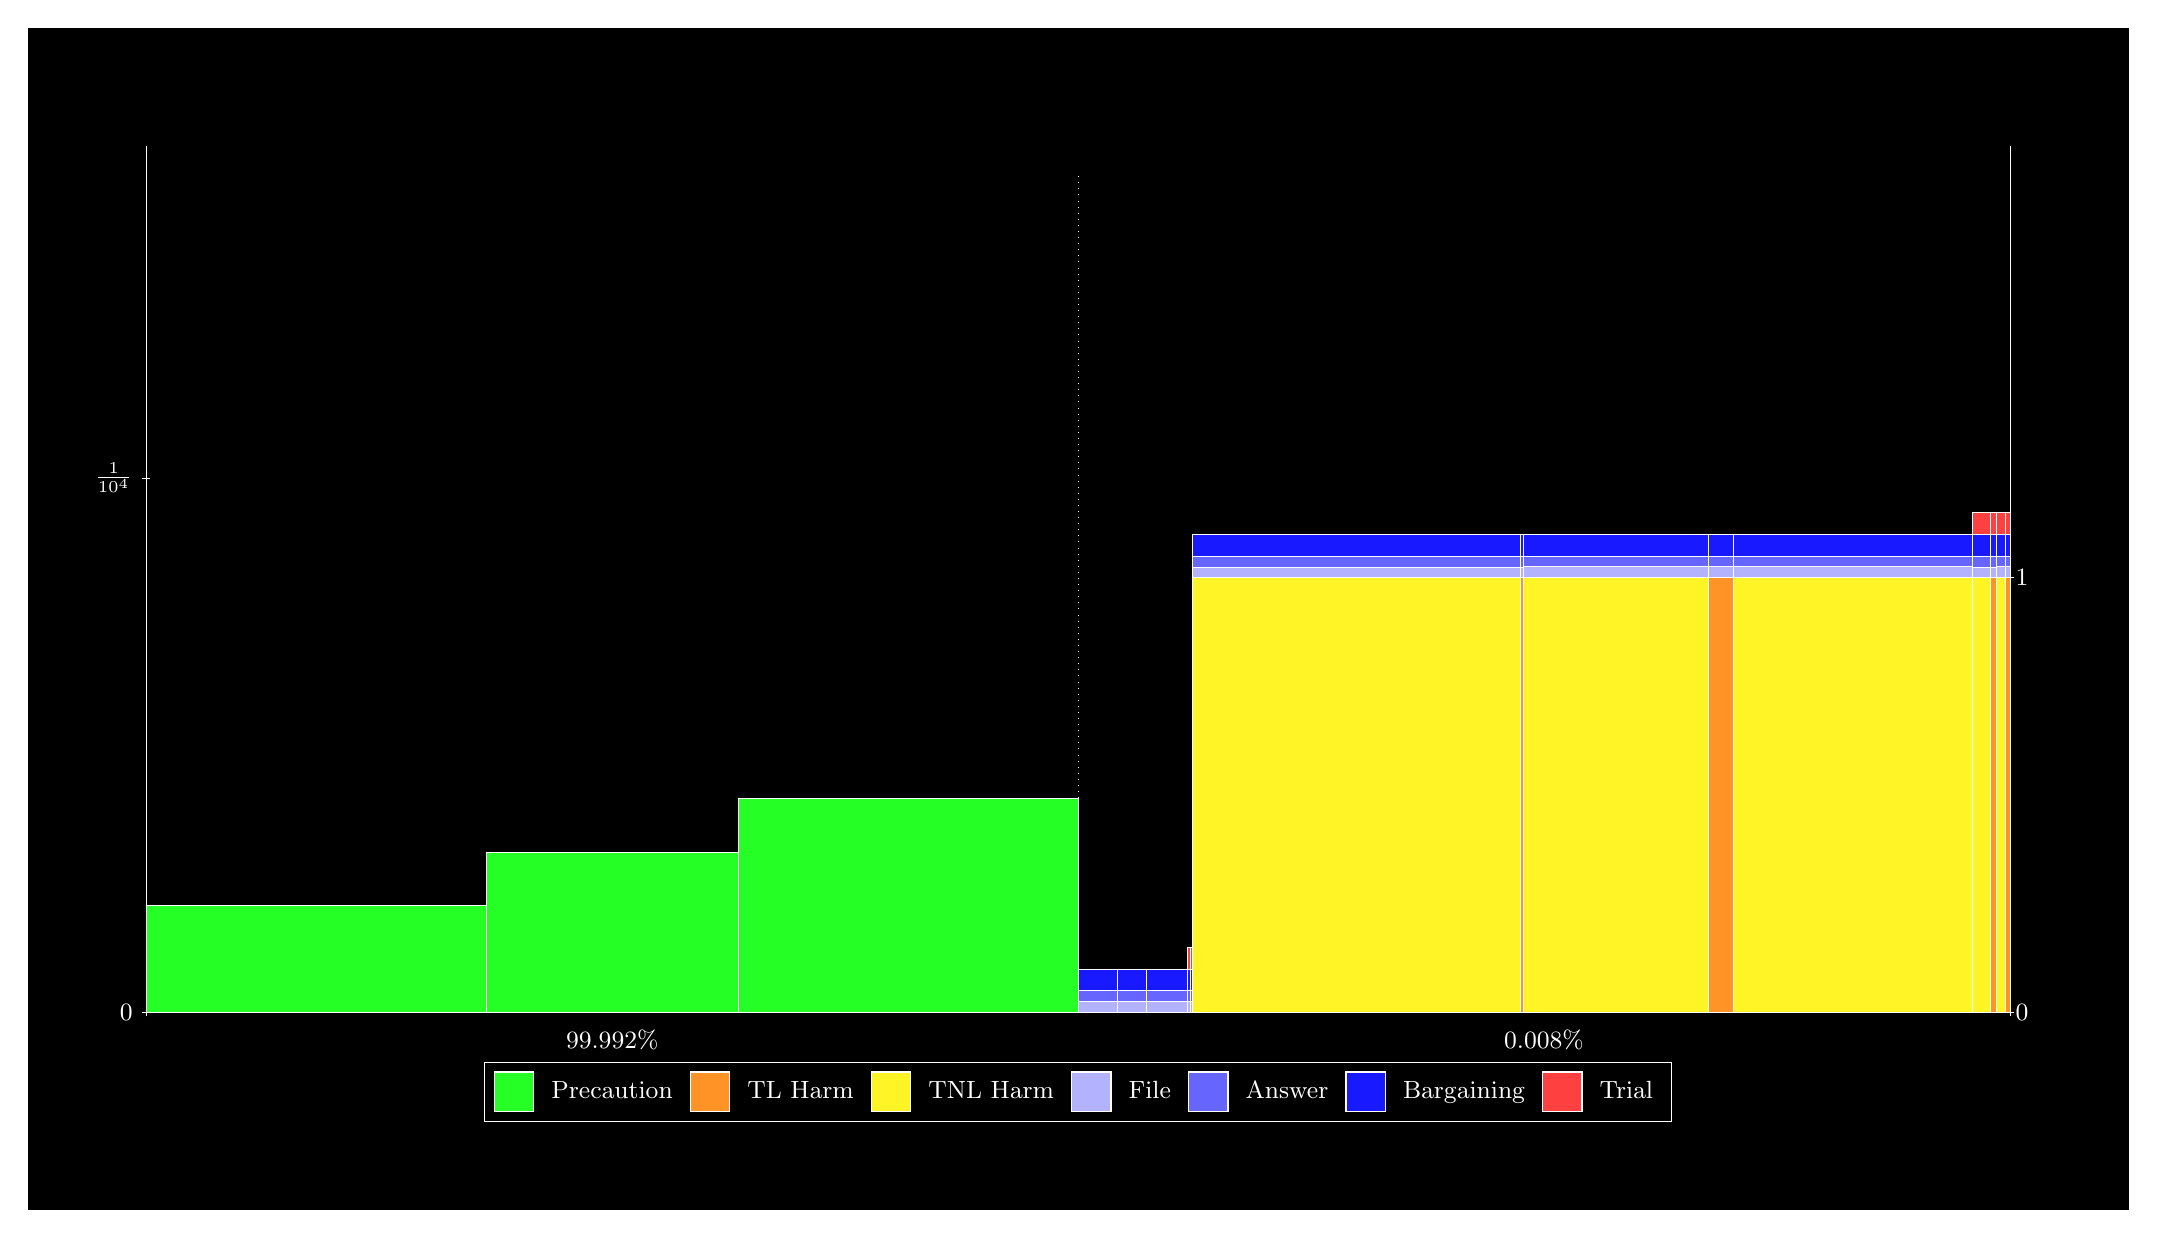
\begin{tikzpicture}
\draw[fill=black] (0,0) rectangle (26.667,15);
\draw[fill=green!85,draw=white,very thin] (1.5,2.5) rectangle (5.8206,3.8576);
\draw[fill=green!85,draw=white,very thin] (5.8206,2.5) rectangle (9.0126,4.5365);
\draw[fill=green!85,draw=white,very thin] (9.0126,2.5) rectangle (13.333,5.2153);
\draw[fill=green!85,draw=white,very thin] (13.333,2.5) rectangle (13.825,2.5001);
\draw[fill=blue!30,draw=white,very thin] (13.333,2.5001) rectangle (13.825,2.6382);
\draw[fill=blue!60,draw=white,very thin] (13.333,2.6382) rectangle (13.825,2.7762);
\draw[fill=blue!90,draw=white,very thin] (13.333,2.7762) rectangle (13.825,3.0523);
\draw[fill=green!85,draw=white,very thin] (13.825,2.5) rectangle (14.193,2.5002);
\draw[fill=blue!30,draw=white,very thin] (13.825,2.5002) rectangle (14.193,2.6382);
\draw[fill=blue!60,draw=white,very thin] (13.825,2.6382) rectangle (14.193,2.7763);
\draw[fill=blue!90,draw=white,very thin] (13.825,2.7763) rectangle (14.193,3.0524);
\draw[fill=green!85,draw=white,very thin] (14.193,2.5) rectangle (14.724,2.5002);
\draw[fill=blue!30,draw=white,very thin] (14.193,2.5002) rectangle (14.724,2.6383);
\draw[fill=blue!60,draw=white,very thin] (14.193,2.6383) rectangle (14.724,2.7763);
\draw[fill=blue!90,draw=white,very thin] (14.193,2.7763) rectangle (14.724,3.0524);
\draw[fill=green!85,draw=white,very thin] (14.724,2.5) rectangle (14.763,2.5001);
\draw[fill=blue!30,draw=white,very thin] (14.724,2.5001) rectangle (14.763,2.6382);
\draw[fill=blue!60,draw=white,very thin] (14.724,2.6382) rectangle (14.763,2.7762);
\draw[fill=blue!90,draw=white,very thin] (14.724,2.7762) rectangle (14.763,3.0523);
\draw[fill=red!75,draw=white,very thin] (14.724,3.0523) rectangle (14.763,3.3284);
\draw[fill=green!85,draw=white,very thin] (14.763,2.5) rectangle (14.788,2.5002);
\draw[fill=blue!30,draw=white,very thin] (14.763,2.5002) rectangle (14.788,2.6382);
\draw[fill=blue!60,draw=white,very thin] (14.763,2.6382) rectangle (14.788,2.7763);
\draw[fill=blue!90,draw=white,very thin] (14.763,2.7763) rectangle (14.788,3.0524);
\draw[fill=red!75,draw=white,very thin] (14.763,3.0524) rectangle (14.788,3.3285);
\draw[fill=green!85,draw=white,very thin] (14.788,2.5) rectangle (18.948,2.5001);
\draw[fill=yellow!85,draw=white,very thin] (14.788,2.5001) rectangle (18.948,8.0222);
\draw[fill=blue!30,draw=white,very thin] (14.788,8.0222) rectangle (18.948,8.1603);
\draw[fill=blue!60,draw=white,very thin] (14.788,8.1603) rectangle (18.948,8.2983);
\draw[fill=blue!90,draw=white,very thin] (14.788,8.2983) rectangle (18.948,8.5745);
\draw[fill=green!85,draw=white,very thin] (18.948,2.5) rectangle (18.989,2.5001);
\draw[fill=orange!85,draw=white,very thin] (18.948,2.5001) rectangle (18.989,8.0222);
\draw[fill=blue!30,draw=white,very thin] (18.948,8.0222) rectangle (18.989,8.1603);
\draw[fill=blue!60,draw=white,very thin] (18.948,8.1603) rectangle (18.989,8.2983);
\draw[fill=blue!90,draw=white,very thin] (18.948,8.2983) rectangle (18.989,8.5745);
\draw[fill=green!85,draw=white,very thin] (18.989,2.5) rectangle (21.341,2.5002);
\draw[fill=yellow!85,draw=white,very thin] (18.989,2.5002) rectangle (21.341,8.0223);
\draw[fill=blue!30,draw=white,very thin] (18.989,8.0223) rectangle (21.341,8.1604);
\draw[fill=blue!60,draw=white,very thin] (18.989,8.1604) rectangle (21.341,8.2984);
\draw[fill=blue!90,draw=white,very thin] (18.989,8.2984) rectangle (21.341,8.5745);
\draw[fill=green!85,draw=white,very thin] (21.341,2.5) rectangle (21.655,2.5002);
\draw[fill=orange!85,draw=white,very thin] (21.341,2.5002) rectangle (21.655,8.0223);
\draw[fill=blue!30,draw=white,very thin] (21.341,8.0223) rectangle (21.655,8.1604);
\draw[fill=blue!60,draw=white,very thin] (21.341,8.1604) rectangle (21.655,8.2984);
\draw[fill=blue!90,draw=white,very thin] (21.341,8.2984) rectangle (21.655,8.5745);
\draw[fill=green!85,draw=white,very thin] (21.655,2.5) rectangle (24.683,2.5002);
\draw[fill=yellow!85,draw=white,very thin] (21.655,2.5002) rectangle (24.683,8.0224);
\draw[fill=blue!30,draw=white,very thin] (21.655,8.0224) rectangle (24.683,8.1604);
\draw[fill=blue!60,draw=white,very thin] (21.655,8.1604) rectangle (24.683,8.2985);
\draw[fill=blue!90,draw=white,very thin] (21.655,8.2985) rectangle (24.683,8.5746);
\draw[fill=green!85,draw=white,very thin] (24.683,2.5) rectangle (24.924,2.5001);
\draw[fill=yellow!85,draw=white,very thin] (24.683,2.5001) rectangle (24.924,8.0222);
\draw[fill=blue!30,draw=white,very thin] (24.683,8.0222) rectangle (24.924,8.1603);
\draw[fill=blue!60,draw=white,very thin] (24.683,8.1603) rectangle (24.924,8.2983);
\draw[fill=blue!90,draw=white,very thin] (24.683,8.2983) rectangle (24.924,8.5745);
\draw[fill=red!75,draw=white,very thin] (24.683,8.5745) rectangle (24.924,8.8506);
\draw[fill=green!85,draw=white,very thin] (24.924,2.5) rectangle (24.998,2.5001);
\draw[fill=orange!85,draw=white,very thin] (24.924,2.5001) rectangle (24.998,8.0222);
\draw[fill=blue!30,draw=white,very thin] (24.924,8.0222) rectangle (24.998,8.1603);
\draw[fill=blue!60,draw=white,very thin] (24.924,8.1603) rectangle (24.998,8.2983);
\draw[fill=blue!90,draw=white,very thin] (24.924,8.2983) rectangle (24.998,8.5745);
\draw[fill=red!75,draw=white,very thin] (24.924,8.5745) rectangle (24.998,8.8506);
\draw[fill=green!85,draw=white,very thin] (24.998,2.5) rectangle (25.109,2.5002);
\draw[fill=yellow!85,draw=white,very thin] (24.998,2.5002) rectangle (25.109,8.0223);
\draw[fill=blue!30,draw=white,very thin] (24.998,8.0223) rectangle (25.109,8.1604);
\draw[fill=blue!60,draw=white,very thin] (24.998,8.1604) rectangle (25.109,8.2984);
\draw[fill=blue!90,draw=white,very thin] (24.998,8.2984) rectangle (25.109,8.5745);
\draw[fill=red!75,draw=white,very thin] (24.998,8.5745) rectangle (25.109,8.8506);
\draw[fill=green!85,draw=white,very thin] (25.109,2.5) rectangle (25.167,2.5002);
\draw[fill=orange!85,draw=white,very thin] (25.109,2.5002) rectangle (25.167,8.0223);
\draw[fill=blue!30,draw=white,very thin] (25.109,8.0223) rectangle (25.167,8.1604);
\draw[fill=blue!60,draw=white,very thin] (25.109,8.1604) rectangle (25.167,8.2984);
\draw[fill=blue!90,draw=white,very thin] (25.109,8.2984) rectangle (25.167,8.5745);
\draw[fill=red!75,draw=white,very thin] (25.109,8.5745) rectangle (25.167,8.8506);
\draw[white,very thin] (1.5,2.5) -- (1.5,13.5);
\draw[white,very thin] (1.45,2.5) -- (1.55,2.5);
\node[font=\small,text=white, anchor=east] at (1.45, 2.5) {0};
\draw[white,very thin] (1.45,9.2882) -- (1.55,9.2882);
\node[font=\small,text=white, anchor=east] at (1.45, 9.2882) {$\frac{1}{10^{4}}$};

\draw[white,dotted,very thin] (13.333,2.83) -- (13.333,13.17);
\draw[white,very thin] (25.167,2.5) -- (25.167,13.5);
\draw[white,very thin] (25.117,2.5) -- (25.217,2.5);
\node[font=\small,text=white, anchor=west] at (25.117, 2.5) {0};
\draw[white,very thin] (25.117,8.0221) -- (25.217,8.0221);
\node[font=\small,text=white, anchor=west] at (25.117, 8.0221) {1};

\draw[white,very thin] (1.5,2.5) -- (25.167,2.5);
\draw[white,very thin] (1.5,2.45) -- (1.5,2.55);
\node[font=\small,text=white, anchor=north] at (1.5, 2.45) {};
\draw[white,very thin] (25.167,2.45) -- (25.167,2.55);
\node[font=\small,text=white, anchor=north] at (25.167, 2.45) {};

\node[font=\small,text=white,anchor=south] at (7.4167, 1.9) {99.992\%};
\node[font=\small,text=white,anchor=south] at (19.25, 1.9) {0.008\%};
\draw (13.3333,2.5) node (B) {};
\begin{scope}[align=center]
\matrix[scale=0.5,draw=white,below=0.5cm of B,nodes={draw},column sep=0.1cm]{
\node[rectangle,draw,minimum width=0.5cm,minimum height=0.5cm,fill=green!85]{}; & \node[draw=none,font=\small,text=white]{Precaution}; &
\node[rectangle,draw,minimum width=0.5cm,minimum height=0.5cm,fill=orange!85]{}; & \node[draw=none,font=\small,text=white]{TL Harm}; &
\node[rectangle,draw,minimum width=0.5cm,minimum height=0.5cm,fill=yellow!85]{}; & \node[draw=none,font=\small,text=white]{TNL Harm}; &
\node[rectangle,draw,minimum width=0.5cm,minimum height=0.5cm,fill=blue!30]{}; & \node[draw=none,font=\small,text=white]{File}; &
\node[rectangle,draw,minimum width=0.5cm,minimum height=0.5cm,fill=blue!60]{}; & \node[draw=none,font=\small,text=white]{Answer}; &
\node[rectangle,draw,minimum width=0.5cm,minimum height=0.5cm,fill=blue!90]{}; & \node[draw=none,font=\small,text=white]{Bargaining}; &
\node[rectangle,draw,minimum width=0.5cm,minimum height=0.5cm,fill=red!75]{}; & \node[draw=none,font=\small,text=white]{Trial}; \\\\
};\end{scope}

\end{tikzpicture}
\end{document}